\begin{figure}[t]
  \hspace{0.05\textwidth}%
  \begin{subfigure}[b]{\textwidth}
    \tikzstyle{legend-point}=[circle, inner sep=2pt]
    \definecolor{legend1}{HTML}{4c72b0}
    \definecolor{legend2}{HTML}{55a868}
    \definecolor{legend3}{HTML}{c44e52}
    \definecolor{legend4}{HTML}{8172b2}
    \definecolor{legend5}{HTML}{ccb974}
    
    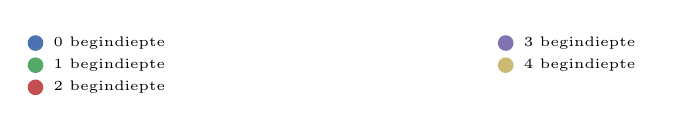
\begin{tikzpicture}
      \node (legend1) at (0.1\textwidth, 0)
            [legend-point, fill={legend1}, label=right:{\tiny $0$ begindiepte}] {};
      \node (legend2) at (0.1\textwidth, -8pt)
            [legend-point, fill={legend2}, label=right:{\tiny $1$ begindiepte}] {};
      \node (legend3) at (0.1\textwidth, -16pt)
            [legend-point, fill={legend3}, label=right:{\tiny $2$ begindiepte}] {};
      \node (legend6) at (0.5925\textwidth, 0)
            [legend-point, fill={legend4}, label=right:{\tiny $3$ begindiepte}] {};
      \node (legend7) at (0.5925\textwidth, -8pt)
            [legend-point, fill={legend5}, label=right:{\tiny $4$ begindiepte}] {};
    \end{tikzpicture}
  \end{subfigure}\hfill\\
  \begin{minipage}[t]{0.5\textwidth}
  \begin{adjustbox}{minipage=\textwidth, scale=0.55}
    \begin{subfigure}[b]{1.6\textwidth}
      \centering
      \def\svgwidth{\textwidth}
      \input{./img/raw/hs-sd-construction-time/construction_sd_time_spaceship-indoor.pdf_tex}
      \caption{Spaceship indoor}
      \vspace{4pt}
      \label{fig:hs-sd-construction:indoor}
    \end{subfigure}
  \end{adjustbox} \\
  %
  \begin{adjustbox}{minipage=\textwidth, scale=0.55}
    \begin{subfigure}[b]{1.6\textwidth}
      \centering
      \def\svgwidth{\textwidth}
      \input{./img/raw/hs-sd-construction-time/construction_sd_time_pipers-alley.pdf_tex}
      \caption{Pipers Alley}
      \vspace{4pt}
      \label{fig:hs-sd-construction:alley}
    \end{subfigure}
  \end{adjustbox} \\
  %
  \begin{adjustbox}{minipage=\textwidth, scale=0.55}
    \begin{subfigure}[b]{1.6\textwidth}
      \centering
      \def\svgwidth{\textwidth}
      \input{./img/raw/hs-sd-construction-time/construction_sd_time_ziggurat-city.pdf_tex}
      \caption{Ziggurat stad}
      \label{fig:hs-sd-construction:city}
    \end{subfigure}
  \end{adjustbox}
  \caption{\small Constructietijd van de Hashed datastructuren bij verschillende startdiepte.}
  \label{fig:hs-sd-construction}
  \end{minipage}%
  %
  \begin{minipage}[t]{0.5\textwidth}
  \begin{adjustbox}{minipage=\textwidth, scale=0.55}
    \begin{subfigure}[b]{1.6\textwidth}
      \centering
      \def\svgwidth{\textwidth}
      \input{./img/raw/hs-sd-memory/memory_sd_spaceship-indoor.pdf_tex}
      \caption{Spaceship indoor}
      \vspace{4pt}
      \label{fig:hs-sd-memory::indoor}
    \end{subfigure}
  \end{adjustbox} \\
  %
  \begin{adjustbox}{minipage=\textwidth, scale=0.55}
    \begin{subfigure}[b]{1.6\textwidth}
      \centering
      \def\svgwidth{\textwidth}
      \input{./img/raw/hs-sd-memory/memory_sd_pipers-alley.pdf_tex}
      \caption{Pipers Alley}
      \vspace{4pt}
      \label{fig:hs-sd-memory:alley}
    \end{subfigure}
  \end{adjustbox} \\
  %
  \begin{adjustbox}{minipage=\textwidth, scale=0.55}
    \begin{subfigure}[b]{1.6\textwidth}
      \centering
      \def\svgwidth{\textwidth}
      \input{./img/raw/hs-sd-memory/memory_sd_ziggurat-city.pdf_tex}
      \caption{Ziggurat stad}
      \label{fig:hs-sd-memory:city}
    \end{subfigure}
  \end{adjustbox}
  \caption{\small Gesommeerd aantal pixels in de texturen van de texturen van de Hashed datastructuren.}
  \label{fig:hs-sd-memory}
  \end{minipage} 
\end{figure}

